\clearpage
\section{Introduction}

AssetWorx \footnote{Pronounced as Asset Works} is a Dutch startup providing a platform for data driven asset management. AssetWorx initially started as GSWRX \footnote{Pronouned as Gas Works}. Working with a variety of medium- to large-sized organizations ranging from government, education to the private sector, GSWRX stimulates disruptive innovation by means of new technologies. One of the parties GSWRX cooperates with is the Dutch province Overijssel during the ‘Startup in Residence’ program. The idea of the startup program is: to develop a new solution in cooperation with a government body, thereby showing product validation and viability by having that respective government body as an early adopter. \cite{Residense2020}.

During this collaboration, GSWRX initiated a platform for Predictive Road Maintenance, with the respective abbreviated name: PRM (see figure \ref{fig:prm}). Recently, GSWRX has pivotted into this specific domain and re-branded the company into AssetWorx.

As of now (Feb. 2021) PRM is only used by the province Overijssel, but AssetWorx is in active negotiation with other provinces and municipalities for adoption. The ultimate goal is to create an uniform data platform for road maintainers. The idea is to be a disrupter of the industry by providing data driven insights in road quality, maintenance and planning as an independent organization (i.e. not a contractor). 

\begin{figure}[ht]
    \begin{center}
    \includegraphics[height=6cm]{images/1_introduction/prm-overview.png}
    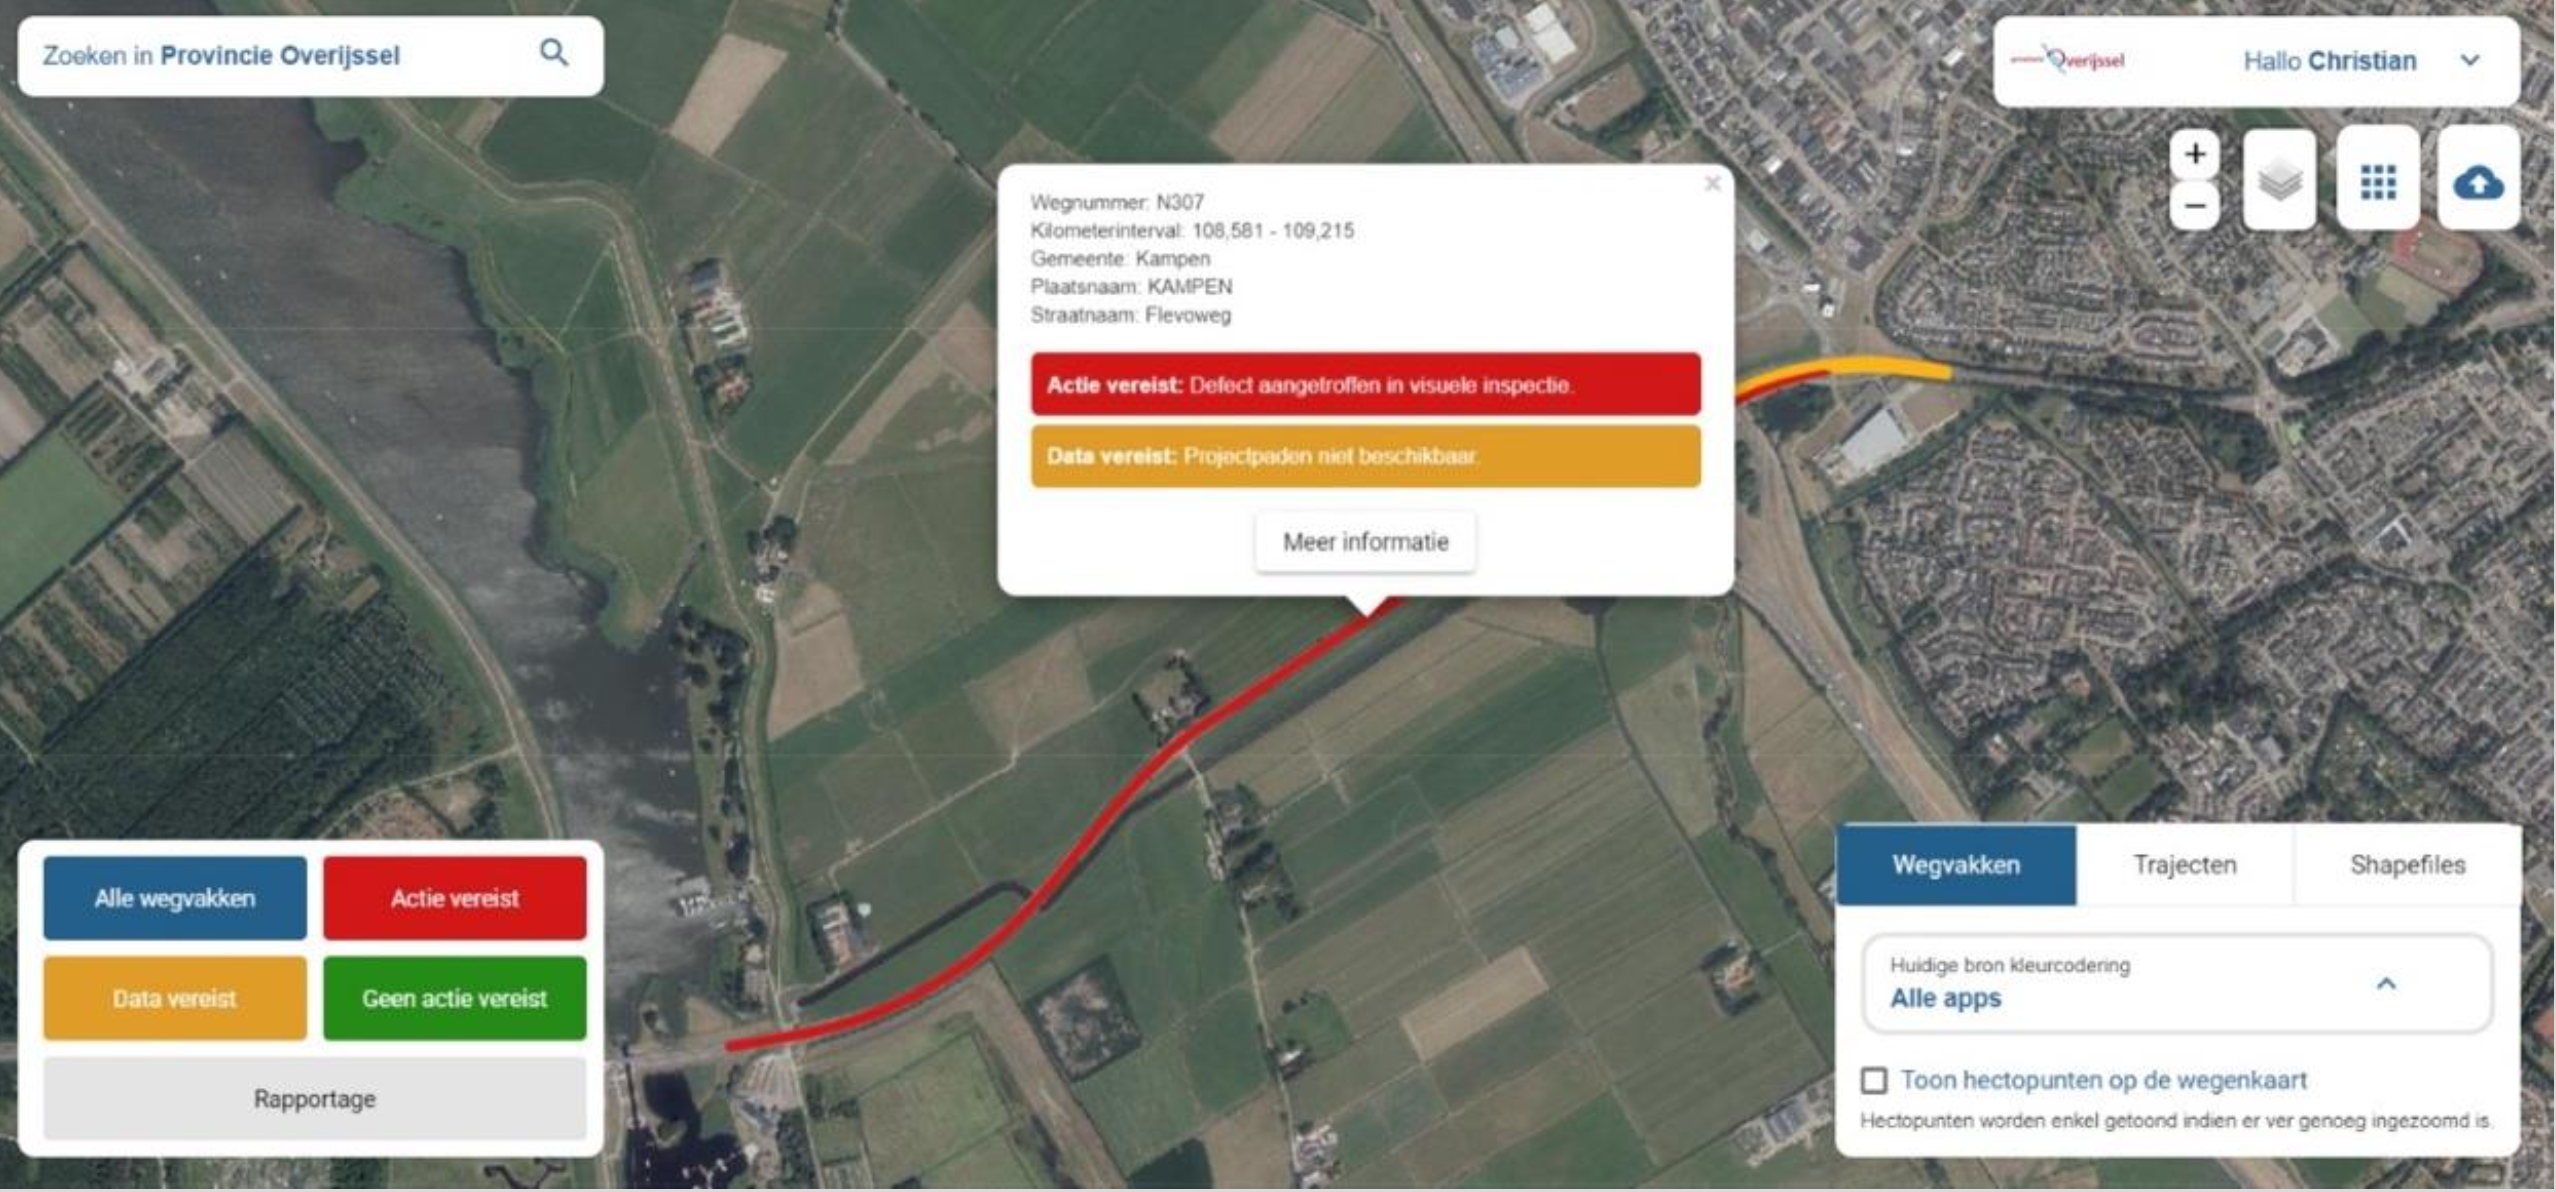
\includegraphics[height=6cm]{images/1_introduction/prm-detail.png}
    \end{center}
    \caption{Screenshots of Predictive Road Maintenance (PRM) software.}
    \label{fig:prm}
\end{figure}

\subsection{Road Surface Defects}

\subsection{Road Maintenance in the Netherlands}

\subsection{Problem Statement}

In the Netherlands, public infrastructure maintainers (the state, provinces, municipalities and water authorities) have the legal responsibility for maintaining their assets \cite{Wegenwet}. Road maintenance is performed through a multi-year plan, which is part of the larger domain of road management. Programming for multi-year road maintenance requires clear insights in current road condition (damages and maintenance status).

Before PRM, there was not a platform integrating \textit{all} the diverse kinds of data collected to assess road's condition. There are solutions which integrates one or two types of data. Example of collected data include visual inspections, automatic measurements and historical reports. These various types of data are later described below in more detail. In order to assess the road condition, the data needs to be manually interpreted and combined. This is an intensive procedure which largely relies on experience and intuition of the inspectors and planners.

\subsection{Research Questions}

In the literature there is already a lot known on road surface defects detection. However, most existing literature focuses on using a single source of data (e.g. visual). In this case we are collecting various types of data (visual + sound + accelerations + CAN). With that in mind, this thesis aims to answer the following research question:

How can we fuse various types of data to enhance road surface defects detection?

Backed by the following sub-questions:
\begin{enumerate}
\item What kind of data and algorithms are generally used in road surface defects detection?
\item What is the state of art in multimodal data fusion?
\item Has mutimodal data fusion been applied to road surface defects? If so, how?
\end{enumerate}

Literature to answer these questions will be gathered with the following procedure:
\begin{enumerate}
\item List search relevant search terms.
\item Find synonyms in a thesaurus.
\item Search literature on Google Scholar \cite{scholar}, Science Direct \cite{science-direct} and Papers with Code \cite{paperswithcode}. 
\item Select potential interesting papers based on their title and abstract.
\item Check Google Scholar which cite the respective paper to see if a more recent version exists (forward citation).
\item Scan through paper references if a specific title seems relevant (backward citation), repeat from 4.
\end{enumerate}


\subsection{Remainder}